\chapter[Introdução]{Introdução}
Este documento traz o relatório do desenvolvimento de ferramenta web utilizando a linguagem python e o framework Flask, para a manutenção remota dos equipamentos de Loterias e ATM's da caixa. 

A Ferramenta possibilita o envio e execução de tarefas de manutenção pré-determinadas aos equipamentos do parque, possibilitando que o usuário do sistema consiga efetuar tarefas de manutenção sem um acesso direto ao equipamento e sem que o usuário tenha a necessidade de ter conhecimento de comandos linux ou mesmo de uso do sistema operacional. 

O sistema permite o agendamento de tarefas utilizando a API Fabric e Celery possibilita a manutenção contínua, geração de imagens e gerência de configurações em um parque de 130 mil máquinas, utilizando toda a filosofia DEVOPs.

O desenvolvimento e planejamento das atividades está apresentada na figura \ref{fig:cronograma}
\section{Cronograma}
\begin{center}
    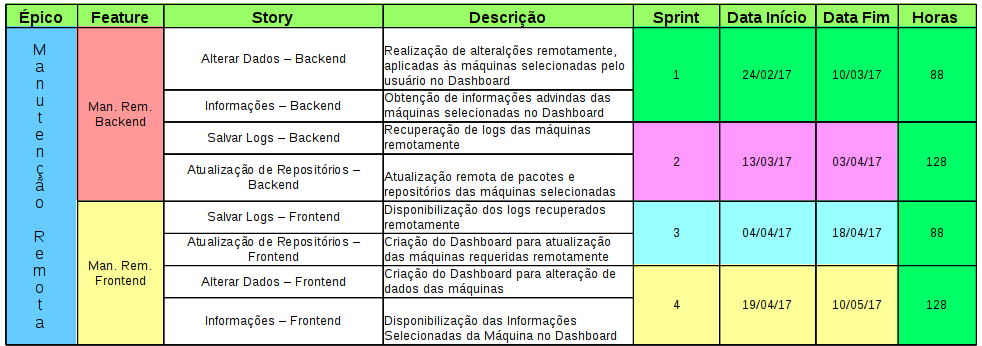
\includegraphics[scale=0.6,angle=90]{figuras/cronograma.png}
    \label{fig:cronograma}
\end{center}
